\documentclass[solution, letterpaper]{cs121}

\usepackage{tikz-qtree}
\usepackage{graphicx}

%% Please fill in your name and collaboration statement here.
%\newcommand{\studentName}{Renzo Lucioni and Daniel Broudy}
%\newcommand{\collaborationStatement}{I collaborated with...}
\newcommand{\solncolor}{red}
\begin{document}

\header{3}{March 15, 2013, at 12:00 PM}{}{}

%%%%%%%%%%%%%%%%%%%%%%%%%%%%%%%%%%%%%%%%%%%%%%%%%%%%
\problem{20} %1
\subproblem %a
% 2epsilon to the m
%width of the range is 2epsilon then for m dimensions
To do this problem i will first ignore the fact that it is a M dimensional hypercube and the just repeat the probability M times. We know that {\bf x} is in the center, we then chose a {\bf y}, what is the probability that it is within $\epsilon$ of {\bf x}. The range that it is to be within is a range of $2\epsilon$, because it can be within $\epsilon$ in either direction. That makes the 1-dimentional probability, $2\epsilon$ we then repeat that in M dimensions and get the probability is $(2\epsilon)^{M}$.


%To do this problem we will first ignore the fact that it is a M dimensional hypercube and instead consider the 1 dimensional case then repeat it M times. First what do we know. We know that $x_m$ and $y_m$ are each some number uniformly chosen between 0 and 1 inclusive. We are then looking at the absolute value of their difference. Because these are both drawn from a uniform distribution we know the absolute value of their difference will give us another distribution. This distribution will be a triangle distribution from zero to 1 that peaks at 0.5 . Now that we have our distribution we can think what is the probability that the absolute value of the difference will be between zero and one. To find this probability we integrate our triangle function between zero and one. This integration is easy because it is triangular. We find the probability that the $max_m \| x_m-y_m \| \leq \epsilon $ for the 1-dimensional hypercube to be 1/2. To then apply this to the $M$-dimensional hypercube we just have to think of applying this probability $M$ times to find the probability that in each dimension $max_m \| x_m-y_m \| \leq \epsilon $. If you do this you get $(1/2)^M$.

\subproblem %b
%pick one then the other has that chance of being within range, at most because maybe the first one you pick is closer to the edge of the hypercube so you don't have as much room to work with.
In this case just think of it like we pick one and then pick the other, the first one we pick is like {\bf x} and the second one we pick is like {\bf y}. {\bf y} has a chance of at most $p$ of being in a range of $\epsilon$ of {\bf x}. This probability could be less that $p$ because if the first value you pick is towards the edge of the M-dimensional unit hypercube then the space that the other value can be in is reduced, this would cause the probability to be less than $p$ but it remains true that the probability that $max_m\| x_m - y_m \| \leq \epsilon$ is at most $p$

\subproblem %c
Euclidian distance for these two points can be defined as 
\begin{eqnarray}
 \|\| {\bf x - y} \|\| = \sqrt{\sum\limits_{i=1}^M (x_m - y_m)^2}  \nonumber   
%x_m - y_m > (x_m - y_m)^2  \\
%x_m - y_m = \sqrt{(x_m - y_m)^2}  \\
%x_m - y_m \leq \sqrt{(x_m - y_m)^2 + \alpha} \tab  \alpha \geq 0 
\end{eqnarray}
%We know (1) to be true because the difference between $x_m$ and $y_m$ is some number between 1 and -1 that when you square it will be smaller and positive.\\
%We know (2) to be true by definition.\\
%We know (3) to be true because the square root of a bigger number is bigger, even for numbers between 0 and 1. 

\begin{eqnarray}
max_m \| x_m-y_m \| =  max_m \| x_m-y_m \| \\
%max_m \| x_m-y_m \| + \alpha \geq  max_m \| x_m-y_m \|  \tab \alpha \geq 0\\
\sqrt{(max_m \| x_m-y_m \|)^2} = max_m \| x_m-y_m \| \\
%\sqrt{\left(\sum\limits_{all other M}^M (x_m - y_m)^2 \right) + (x_m + y_m)^2}  \geq  max_m \| x_m-y_m \| \\
\sum\limits_{i=1}^M (x_m - y_m)^2 \geq (max_m \| x_m-y_m \|)^2 \\
\sqrt{\sum\limits_{i=1}^M (x_m - y_m)^2}  \geq  max_m \| x_m-y_m \| \\
\|\| {\bf x - y} \|\|  \geq  max_m \| x_m-y_m \| 
\end{eqnarray}

From these equations it is clear that $\|\| {\bf x - y} \|\|  \geq  max_m \| x_m-y_m \| $ if this is true then the probability that $\|\| {\bf x - y} \|\| \leq \epsilon$ is also at most $p$, this is clearly true because the we just proved that for any two points the euclidian distances is $\geq  max_m \| x_m-y_m \| $ therefore any two points are even less likely to be within a euclidian distance of $\epsilon$ then they are to be with in a 1-dimensional distance of $\epsilon$. This means they cannot have a greater probability of being within a distance of $\epsilon$ of each other, only a equal or lesser chance. therefore $\|\| {\bf x - y} \|\| \leq \epsilon$ is also at most $p$

\subproblem %d  \delta is just a parameter, 
Now we must find the lower bound on the number $N$ of points needed to guarantee, with a probability of at least 1-$\delta$, that the nearest neighbor of a newly selected point $x$ is within a radius $\epsilon$. 

Well we know the probability that some other point is within $\epsilon$ is $(2\epsilon)^M$. 

We know that the probability that two points are not within $\epsilon$ of each other is 1-p

The probability that N points are not within epsilon is $(1-p)^N$. so we set $(1-p)^N = \delta$ to solve this expression we take the log of both sides. 

\[log((1-p)^N) =log( \delta)\]
\[ N =\frac{log( \delta)}{log((1-p))}\]

We can determine that this N is a minimum because as you increase the number of points you increase the chance that a near neighbor would exist. Therefore this equation lays out a minimum value for N to have the probability be at least 1-$\delta$
%Because $p$ is a maximum, this expression for N is actually a minimum because $p$ could be smaller in which case N wouldn't have to be as big to be equal to $\delta$ in the above expression. So in the end you want an N greater than the expression on the right.
\[ N \geq \frac{log( \delta)}{log((1-(2\epsilon)^M))}\]

\subproblem %e we can conclude it is not good.
We can conclude that the HAC algorithm is not very effective on high dimensional spaces. As we discussed in lecture HAC fails on high dimensional data due to what is called the curse of dimensionality. One of the negative sides of the HAC algorithm is that it depends on the inter-point distances. As we can see from our calculations as the dimension M increases the number of points you need to have to guarantee that points are within $\epsilon$ of each other with some probability 1-$\delta$ increases dramatically.  

%%%%%%%%%%%%%%%%%%%%%%%%%%%%%%%%%%%%%%%%%%%%%%%%%%%%
\problem{25}  %2

\subproblem %a
%http://en.wikipedia.org/wiki/Posterior_probability
%Posterior Probability is preportional to Prior Probability * Likelihood 

%\[ Pr( \theta \| D ) = \frac{Pr(\theta)Pr(D \| \theta)}{ \int_{-\infty}^{\infty} Pr(\theta)Pr(D \| \theta)}\]
%\[ Pr({\bf x} \| D ) = \frac{Pr(\theta)Pr(D \| \theta)}{ \int_{-\infty}^{\infty} Pr(\theta)Pr(D \| \theta)}\]

%Predictive Distribution\\

%ML - maximum likelihood
%	TODO FIX THE THETA UNDERNEATH
ML\\
\[  \theta_{ML} = argmax_{\theta} P(D \| \theta)\]
\[PR_{ML}(x \| D) = PR_{ML}(x \| \theta_{ML}) = PR_{ML}(x \| argmax_{\theta} P(D \| \theta)  \]   \\
%MAP - maximum apriori
MAP\\
\[  \theta_{MAP} = argmax_{\theta} P(D \| \theta)p(\theta)\]
\[PR_{ML}(x \| D) = PR_{ML}(x \| \theta_{MAP}) = PR_{ML}(x \| argmax_{\theta} P(D \| \theta)p(\theta)  \] 

%FB - full Bayesian
FB\\
\[PR_{FB}(x \| D) = \int_{\Theta} p(x, \theta)p(\theta \| D) d\theta \]  \\


\subproblem  %b
%more basin because it factors in the prior pr(\theta) this is like factoring in how rare the values could be
% lecture 11 - bottome page 8
MAP method can be consider more bayesian because it factors in prior knowledge to help prevent over fitting. MAP is not fully bayesian because it picks a single set of values for parameters $\theta$ and then uses them for classification and inference as if they are correct, point approximations.


\subproblem %c
%what does MAP enjoy over ML and enjoy over FB methods 
MAP enjoys the benefit of prior knowledge which it can use to penalize setting and attribute that is too unlikely given prior hypotheses. This helps prevent over fitting to the data. MAP enjoys simplicity over the Full Bayesian Method. You don't have to calculate the full posterior distribution. 

\subproblem %d
\begin{center}
  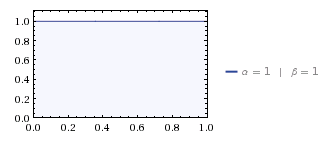
\includegraphics{beta-1-1}
  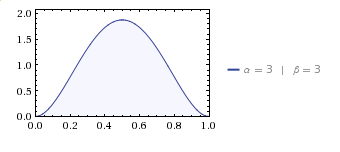
\includegraphics{beta-3-3}
  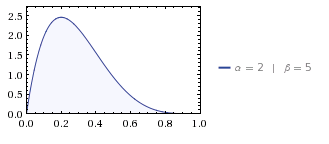
\includegraphics{beta-2-5}
  \end{center}
  
  Beta[1,1] is a uniform prior. this is similar to having had 1 win and 1 loss in the past which is  very little prior information.
  Beta[3,3] is like having more information that you have had more ties, and so you would expect more ties in the future, you have reason to expect a relatively balanced win-loss ratio.
  Beta[2,5] is like having a team that has a record closer to 2-5, so you expect to lean one direction but not all the way one direction. 

\subproblem %e
%COME BACK TO THIS, ask someone else
Beta is the conjugate prior to bernoulli. Beta is between zero and one. Beta takes two parameters. The main reason is Beta distribution's are useful when used together with MAP estimation for reasoning with Bernoulli random variables because the beta distribution is a suitable model for the random behavior of percentages and proportions.

\subproblem %f
Harvard football when 9-1 in the 2011 fall season! 
Harvard football also won their first three games in the 2012 season! We are trying to predict the 4th game of that season.

ML\\
\[ \theta_{ML} = \frac{N_1}{N} = \frac{3}{3} = 1�\]


MAP\\
Given a prior on $\theta$ that is Beta(9,1).\\

\[ \theta_{MAP} = argmax_{\theta} p(\theta \| D) =  \frac{\alpha + N_1 - 1}{ \alpha + \beta + N - 2} = \frac{11}{11}��\]


FB\\

\[ p (x = 1 \| D ) = \int_0^1 p(x=1 \| \theta) p(\theta \| D) d\theta\]

\[  = \int_0^1 \theta \cdot p(\theta \| D) d\theta\]

\[  = E[\theta \| D ] =  \frac{\alpha + N_1}{ \alpha + \beta + N} = \frac{9 + 3}{ 13} = \frac{12}{13}  \]


%%%%%%%%%%%%%%%%%%%%%%%%%%%%%%%%%%%%%%%%%%%%%%%%%%%%
\problem{24}  %3

\subproblem %a
%objective is loss function 
% lecture slides 9 slide 23 just find objective
\[ \L( \{\ \mu_k\}_{k=1}^k , \{r_n\}_{n=1}^N ) = \sum_{n=1}^N \sum_{k=1}^K r_{kn} \|\| x_n - \mu_k \|\|^2 \]

\[ \frac{\delta}{\delta \mu} \L( \{\ \mu_k\}_{k=1}^k , \{r_n\}_{n=1}^N ) = \frac{\delta}{\delta \mu} \sum_{n=1}^N \sum_{k=1}^K r_{kn} \|\| x_n - \mu_k \|\|^2 \]

We can ignore the sums and such for now.
\[  = \frac{\delta}{\delta \mu}  r_{kn} \|\| x_n - \mu_k \|\|^2 \]
we rewrite the $\|\| k_n - \mu_k \|\|^2$ as a dot product
\[  =   r_{kn} \frac{\delta}{\delta \mu}( x_n - \mu_k )\cdot( x_n - \mu_k ) \]

\[  =   r_{kn} \frac{\delta}{\delta \mu} \left( (x_n^1 - \mu_k^1 )^2 + (x_n^2 - \mu_k^2 )^2 + ... \right) \]

\[  =   r_{kn}  \left( (2\mu_k^1 -2x_n^1 ),  (2\mu_k^2 -2x_n^2 ), ...\right) \]

\[  0 =  \sum_{n=1}^N \sum_{k=1}^K r_{kn} \left( (2 (\mu_k - x_n ) \right) \]

now when we want to talk about one $\mu_k$

\[ \sum_{n=1}^N r_{nk}\mu_k - \sum_{n=1}^N r_{nk}x_n = 0 \]

\[   \mu_k = \frac{\sum_{n=1}^N r_{nk}x_n}{\sum_{n=1}^N r_{nk}}  \]


We thus have the update rule for $\mu$

The update rule for $r_{nk}$ cant really be done by taking a partial because it isn't continuous.
Instead we know that only one of the $r_{nk}$ values equals one and we want to minimize the loss function 

\[ \L( \{\ \mu_k\}_{k=1}^k , \{r_n\}_{n=1}^N ) = \sum_{n=1}^N \sum_{k=1}^K r_{kn} \|\| x_n - \mu_k \|\|^2 \]

So you want to pick the $r_{nk}$ that minimizes the loss function by picking the one that corresponds to the  
\[ r_{nk} = argmin_{k^{'}} \|\| x_n - \mu_k^{'} \|\|^2\]



%kmeans clustering objective
%two update steps one for responsibility and one for prototypes 
%take partials that give us these equations found on lecture9slides p20


%show how the update rule can be derived by preforming gradient descent eg. taking a partial wrt/ mew

\subproblem  %b
%k-means is a simple example of an unsupervised algorithm 
% PCA is a well known approach for dimensionality reduction
% PCA is a relaxed solution of k-means clustering.
% in k-means finding distance in the high dimension in PCA we are projecting it down to lower dimensions. 
In some ways you can think of PCA as a relaxed solution to k-means clustering. In k-means we are finding the distance from the mean in a high dimension space, in PCA we are projecting the data down into a set of linearly uncorrected variables called principle components. We know PCA works well for dimensionality reduction. 
k-means is appropriate in dealing with clear categories and clear clusters, if you wanted to separate boys from girls or apples from oranges from bananas, k-means would be very good at categorizing those objects based upon some observations. On the other hand like the example shown in class PCA does well in dealing with images where there are a lot of different colors and shapes that can be projected down into a simpler dimension.


%%%%%%%%%%%%%%%%%%%%%%%%%%%%%%%%%%%%%%%%%%%%%%%%%%%%
\problem{75} %4
\begin{enumerate}
	%%%%%%%%%%%%%%%%%%%%%1.
	\item 
		\begin{enumerate}
			\item The requested graph is below.
				\begin{center}
				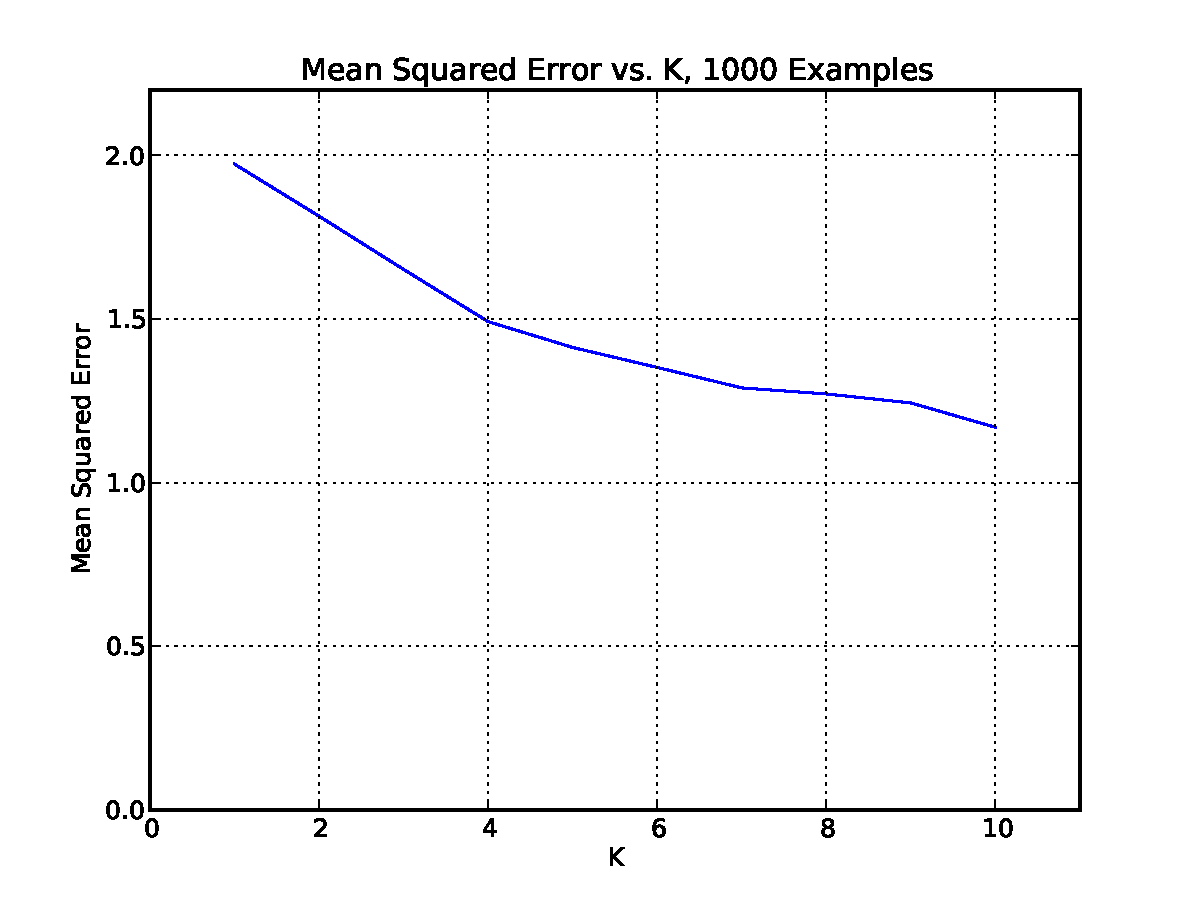
\includegraphics[scale=0.8]{mse-vs-k.pdf}
				\end{center}
			\item If we were to choose the best $K$ for this data based on the plot we generated above, we would choose $K = 8$, since this value of $K$ has a relatively low mean squared error (MSE) without the risk of overcomplicating the model. Choosing a higher value of $K$ will of course result in a lower MSE, but doing this defeats the purpose of clustering, since we are overfitting to the data. In the extreme case, every example in the data will have its own cluster, and the MSE will be 0, but this model does not generalize well.
		\end{enumerate}
	%%%%%%%%%%%%%%%%%%%%% 2.
	\item
		\begin{enumerate}
			\item %a 
			       The requested table and scatterplots are below. \\
				\begin{center}  
				\begin{tabular}{| c | c | c | c | } \hline
				\multicolumn{2}{| c |}{\emph{min}} & \multicolumn{2}{| c |}{\emph{max}}  \\    \hline         
				Cluster & Instances & Cluster& Instances  \\ \hline
				1 & 1 & 1 & 7\\
				2 & 1 & 2 & 35 \\
				3 & 20 & 3 & 21 \\
				4 & 78 & 4 & 37 \\ \hline
				\end{tabular}
				\end{center}
				\hfill \\
				In the following scatterplots, red circles correspond to cluster 1, blue triangles correspond to cluster 2, green squares correspond to cluster 3, and black stars correspond to cluster 4.
				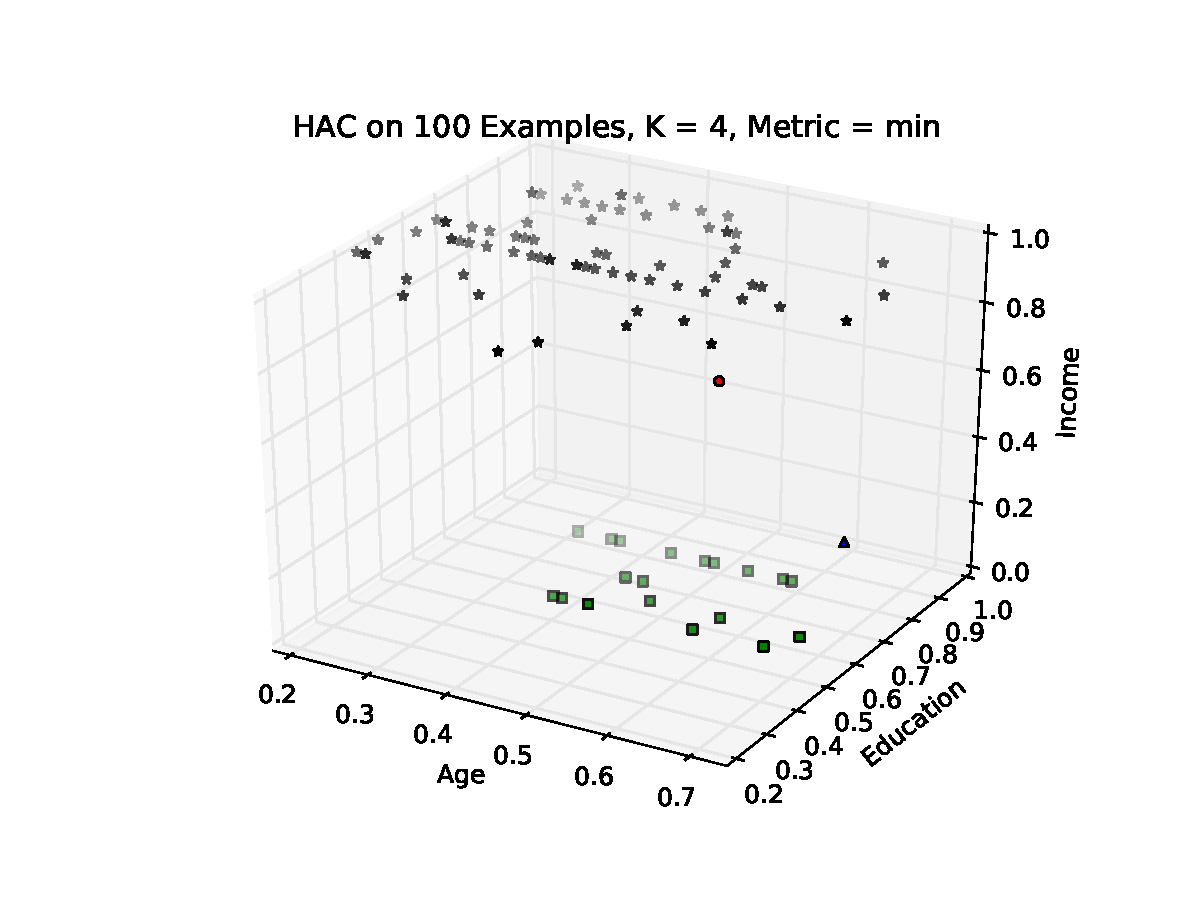
\includegraphics[scale=0.8]{hac-min.pdf}
				
				With the min metric we expect clusters that "snake" from example to example. Min causes the "chaining effect " which we can see in our graph, many of the clusters have the long thin shape you would expect with snaking. Yes this makes sense with the definition of the min metric.\\
				
				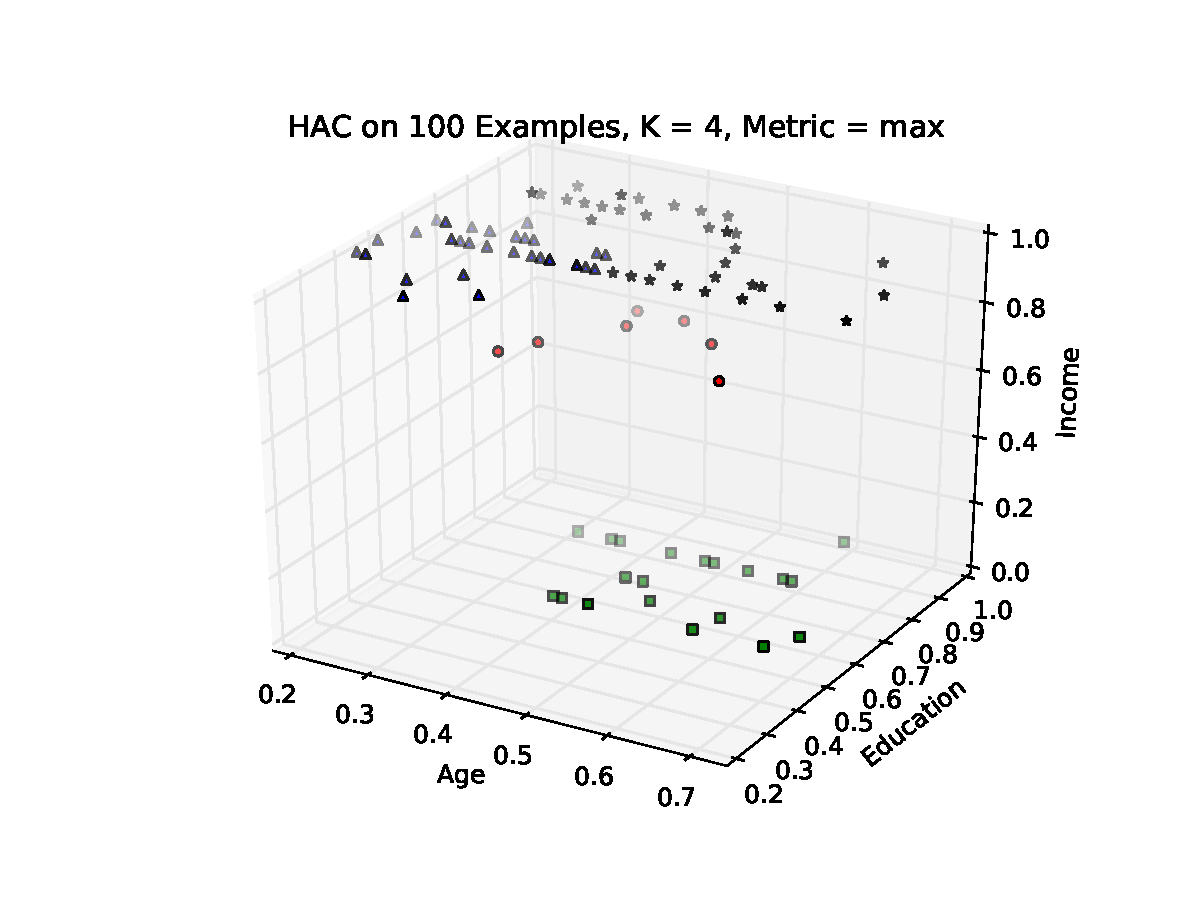
\includegraphics[scale=0.8]{hac-max.pdf} 
				For the max metric we expect clusters to grow in more convex structures than in min. This appears to be more or less true in the graph we produced above.			
			\item %b
			The requested table and scatterplot are below. \\
				\begin{center}  
				\begin{tabular}{| c | c | c | c | } \hline
				\multicolumn{2}{| c |}{\emph{mean}} & \multicolumn{2}{| c |}{\emph{centroid}}  \\    \hline         
				Cluster & Instances & Cluster& Instances  \\ \hline
				1 & 1 & 1 & 1\\
				2 & 26 & 2 & 50 \\
				3 & 50 & 3 & 130 \\
				4 & 123 & 4 & 19 \\ \hline
				\end{tabular}
				\end{center} 
				\hfill \\
				In the following scatterplots, red circles correspond to cluster 1, blue triangles correspond to cluster 2, green squares correspond to cluster 3, and black stars correspond to cluster 4.
				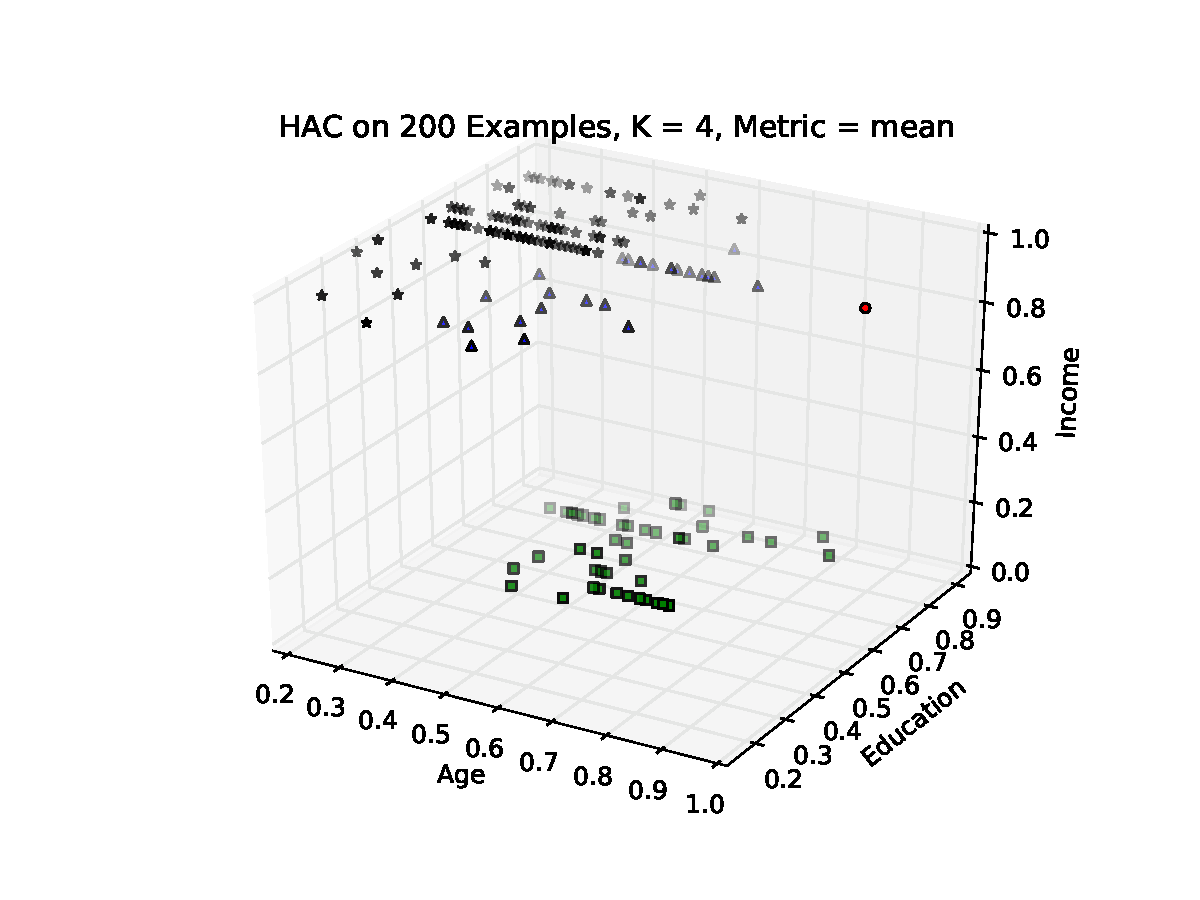
\includegraphics[scale=0.8]{hac-mean.pdf}
				The mean and centroid metrics provide compromises between the min and max metrics 
				
				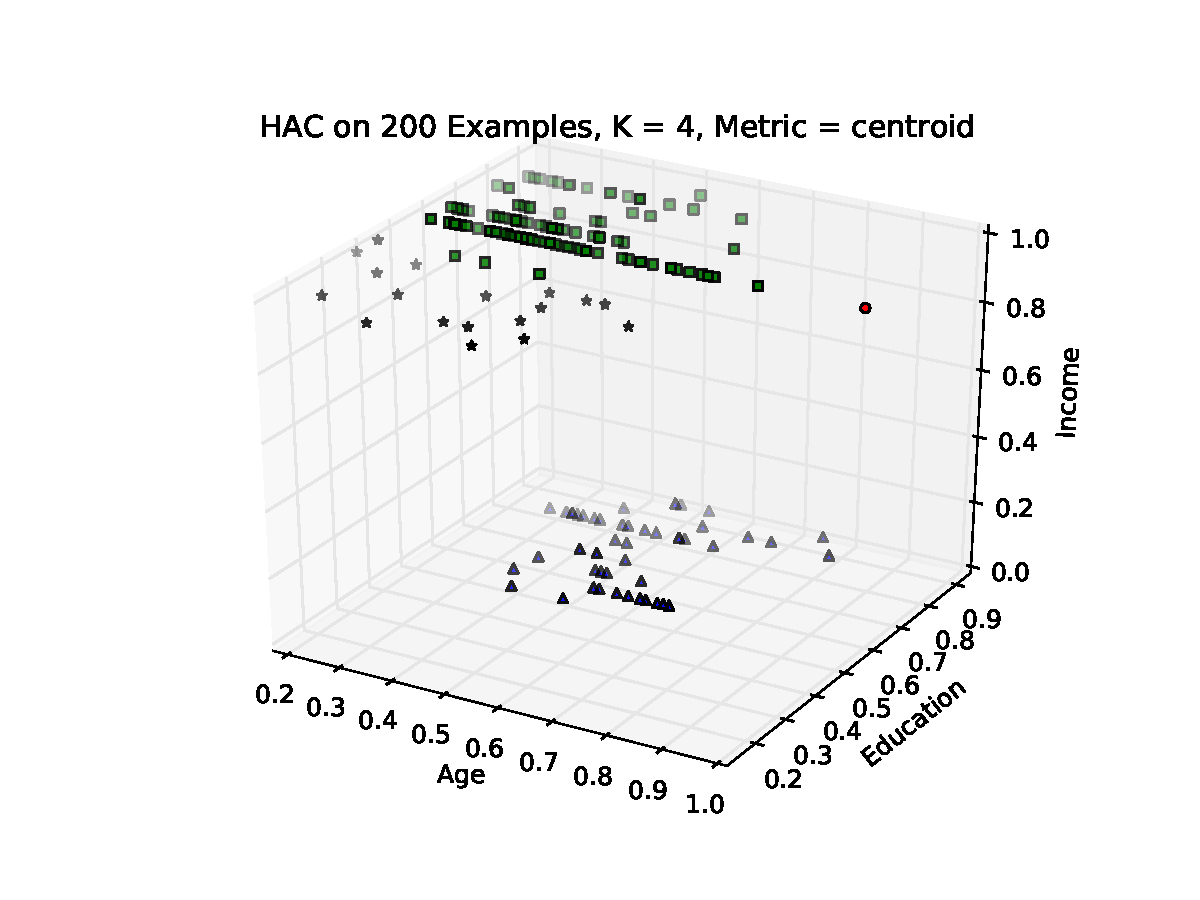
\includegraphics[scale=0.8]{hac-centroid.pdf} 
				We expect the centroid metric to grow convex structures and for those structures to be less affected by outliers. We also expect them to be relatively similar because they are compromises between min and max. This aligns relatively well with what we see in the graph above.
		\end{enumerate}
	%%%%%%%%%%%%%%%%%%%%3.
	\item
		\begin{enumerate}
		\item When run on the {\tt adults} dataset with \emph{numexamples} = 1000 and $K$ = 4, it takes (on average) about 30 iterations for our parameters to converge. 
		\item The requested plot is below:
			\begin{center}
			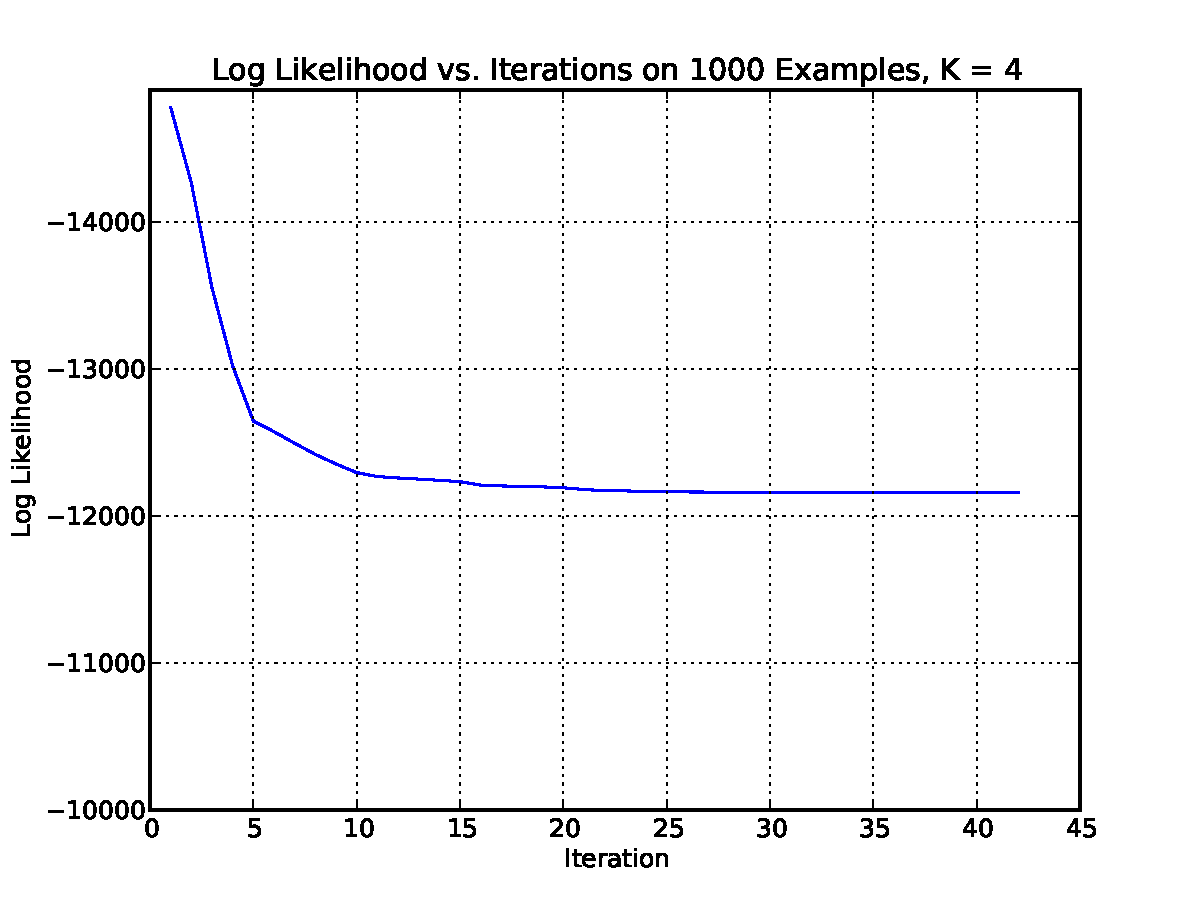
\includegraphics[scale=0.8]{autoclass-likelihoods.pdf} 
			\end{center}
		\item The run-time performance of Autoclass is noticeably worse than that of $K$-means. With $K=4$, $K$-means is capable of running on the entire dataset in approximately 10 seconds, as determined by the Unix {\tt time} utility. However, Autoclass requires about half that time to run on merely 1000 examples, and would take significantly longer than $K$-means to run on the entire dataset.
		\item The requested plot of the log likelihood against $K$ is below.
		\begin{center}
		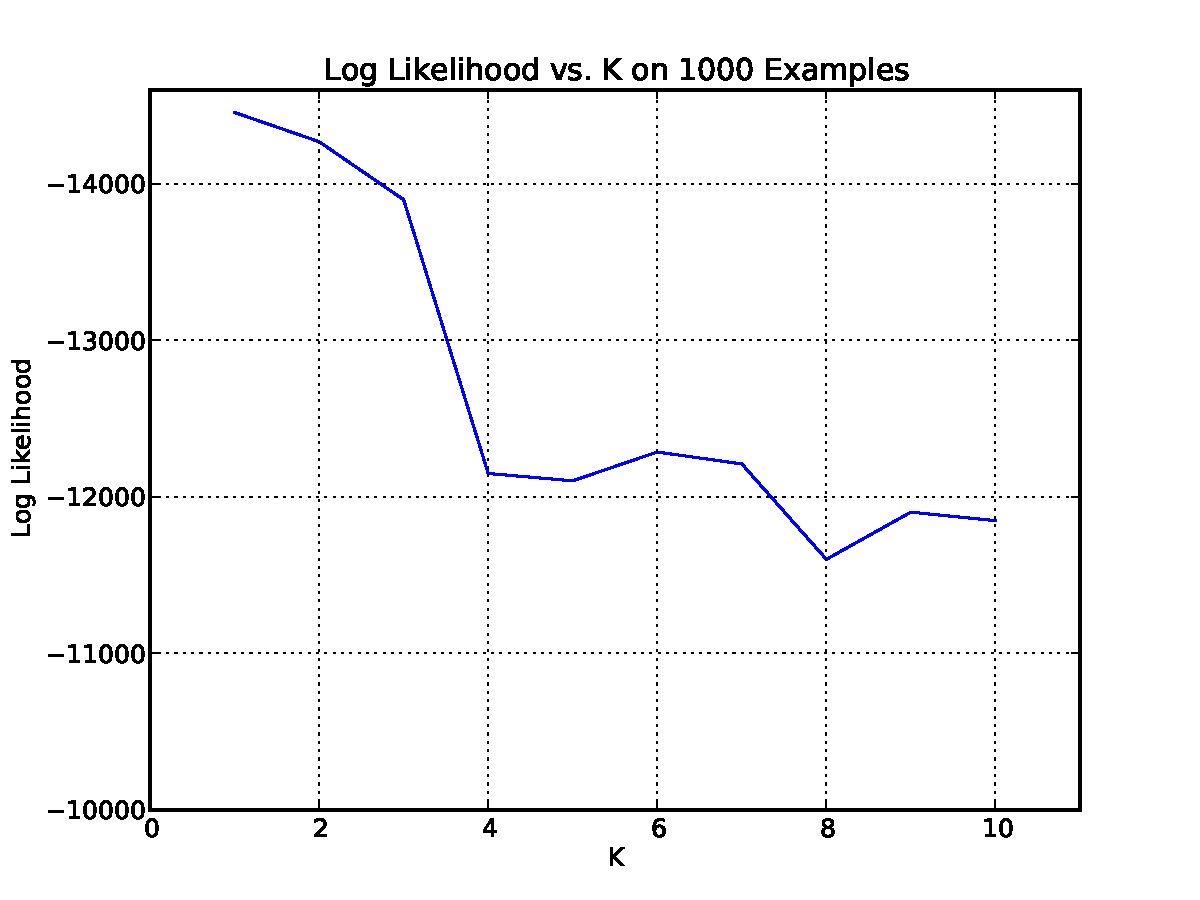
\includegraphics[scale=0.8]{autoclass-likelihoods-v-k.pdf} 
		\end{center}
		If we were to choose the best $K$ for this data, we would choose $K = 8$, since this value of $K$ is associated with a relatively high log likelihood but does not risk overcomplicating the model. Choosing a higher value of $K$ may result in a lower log likelihood, but doing this would make us prone to overfitting the data, giving us a model that may not generalize well.

		\end{enumerate}
\end{enumerate}

\end{document}






